\chapter{Religion, Authority, and Education II}

This chapter follows J. Krishnamurti's San Diego conversation with Dr. Alan W. Anderson on religion, authority, and education. No validated blackboard images, equations, or board diagrams survive for this lecture, so the notes use only transcript-backed schematic diagrams. The argument nevertheless has a definite structure. It begins at the brink of inquiry, where fear and hesitation appear; it traces that hesitation to education in function and measure; it separates freedom from authority; it tests the distinction in the classroom and in the reading of books; and it closes by opening the next question, meditation, as inseparable from conduct, relationship, love, death, and care.

\section{The Brink Of Inquiry}

Anderson begins by returning to the previous conversation. The issue is not a new doctrine but a threshold already reached. In going deeply into oneself, one comes to a point where the mind boggles. There is hesitation, fear, and trembling. Krishnamurti takes this not as an incidental psychological difficulty but as the starting point of the whole conversation: why do we come to the brink and withdraw?

We should read the lecture from that question. The problem is not first whether one has the right belief about religion. The problem is whether the mind can remain with inquiry when inquiry no longer offers comfort, status, or a measurable result.

\begin{align}
\hbox{inquiry}
&\longrightarrow \hbox{brink}
\longrightarrow \hbox{fear and trembling},\\
\hbox{fear and trembling}
&\longrightarrow \hbox{withdrawal}.
\end{align}

These arrows are only a transcript-backed bookkeeping device. They do not turn the conversation into a formal system. They mark the sequence Krishnamurti is asking us to examine: does fear at the edge of inquiry have to end in withdrawal?

\subsection{Question \& Answer}

\paragraph{Question.}
Why do we come to the brink of inquiry and not take the plunge?

\paragraph{Answer.}
Krishnamurti's first answer is educational. We have been trained for function: engineer, professor, doctor, specialist, professional, useful member of a society that measures competence. But the inquiry into religion, freedom, attention, and truth has no comparable measure. When a mind trained by measurable function enters a field where it cannot measure, it hesitates. Not knowing how to proceed, it looks for dependence.

\begin{align}
\hbox{functional training}
&\longrightarrow \hbox{measure}
\longrightarrow \hbox{status}
\longrightarrow \hbox{dependence}
\longrightarrow \hbox{authority}.
\end{align}

So the hesitation is not explained merely by personal timidity. It is tied to a whole training of the mind. We know how to operate where there is a standard of success. We do not know what to do when the inquiry demands all our attention and gives no external yardstick.

\section{Function, Measure, And Status}

Krishnamurti does not dismiss function. Functional knowledge has its place. A society needs engineers, doctors, teachers, crafts, languages, procedures, and skills. The error begins when the structure of function becomes the model for the whole of life, including the field in which one asks what religion, freedom, God, beauty, or truth might mean.

\begin{definition}
In this chapter, \emph{function} means trained operation in a field of knowledge: a profession, a technique, a career, or a socially measurable skill.
\end{definition}

In a functional field, comparison has an obvious role. A calculation may be right or wrong. A bridge may stand or fail. A physician may diagnose well or badly. A student may master or not master a procedure. Krishnamurti's point is that the mind educated almost entirely in that atmosphere carries the same demand for measurement into a field where measurement is not available.

\begin{proposition}
When a mind trained chiefly by measurable function enters an immeasurable inquiry, it tends to substitute authority for direct seeing.
\end{proposition}

\begin{proof}
The argument follows the order of the conversation.
\begin{enumerate}
\item Education gives great importance to function, career, technique, and status.
\item Function is normally assessed by external measures.
\item Religious inquiry, as Krishnamurti uses the phrase, has no such external measure.
\item The mind trained by measure finds itself without its familiar instrument.
\item In that uncertainty, it looks to one who claims to know.
\item The claim of another to know becomes authority.
\end{enumerate}
Thus dependence is not an accidental weakness added later. It is the transfer of a functional habit into a field that requires freedom from the beginning.
\end{proof}

The distinction can be held compactly.

\begin{table}
\centering
\begin{tabular}{p{0.43\linewidth} p{0.43\linewidth}}
Field of knowledge & Field of inquiry \\
\hline
Function, technique, skill & Freedom, attention, direct seeing \\
Measure and comparison & No external measure \\
Instruction has a limited place & Authority obstructs inquiry \\
Thought is necessary & Thought must know its limit \\
\end{tabular}
\end{table}

This table is not a final doctrine. It is a guardrail. Krishnamurti is not saying that knowledge is useless. He is saying that when knowledge, measure, and function become the whole movement of the mind, the capacity to inquire is dulled.

\section{Freedom Before Inquiry}

The next turn is from education to perception. Krishnamurti says that to inquire there must be freedom first. If one comes with prejudice, one cannot inquire. If one comes with a conclusion, one cannot inquire. If one looks through an image, one does not see what is living.

The word ``image'' is important here. One may look at a tree through knowledge, at a person through memory, at nature through translation and enjoyment, or at religion through a book, a priest, or a belief. In each case, the living thing is replaced by something already known.

\begin{align}
\hbox{living thing}
&\longrightarrow \hbox{image, memory, knowledge, translation}\\
&\longrightarrow \hbox{indirect perception}.
\end{align}

The issue is not ordinary ignorance. Krishnamurti is not asking us to forget how to function. He is distinguishing knowledge in its proper field from knowledge as a screen. That distinction prepares the later claim that thought has a necessary place in the field of knowledge but cannot build or reach the timeless.

\subsection{Question \& Answer}

\paragraph{Question.}
Can freedom and authority coexist in religious inquiry?

\paragraph{Answer.}
No. In Krishnamurti's sequence, freedom and authority cannot possibly exist together. Authority may seem useful where one is learning a technique, but in the inquiry into religion, truth, beauty, God, or freedom, authority becomes dependence. Freedom is not promised at the end of obedience; it is required at the beginning.

Krishnamurti then joins freedom to intelligence. Intelligence is not accumulated information. It is linked with sensitivity, attention, perception, and action. Anderson helps bring out the immediacy of the point: perception is intelligence, and perception is the act.

\begin{align}
\hbox{freedom}
&\longrightarrow \hbox{inquiry},\\
\hbox{attention}
&\longrightarrow \hbox{intelligence},\\
\hbox{perception}
&\longrightarrow \hbox{action}.
\end{align}

The danger is that the living relation can be converted into a concept. Anderson notices this immediately: once translated into a concept, even the positive movement of intelligence, beauty, love, truth, freedom, and death can become an occasion for terror. Krishnamurti agrees. The concept is no longer the thing.

\section{The Book, The Class, And The Clean Eye}

The middle of the dialogue brings the inquiry into a classroom. Anderson asks how inherited texts, scriptures, and classical materials can be taught without making the student inwardly divided or second-hand. The teacher must know functional material; the student will read books. But can the book be used without becoming authority?

Krishnamurti reverses the usual order. If he had a class, he says, he would not begin with the book. He would begin with freedom. Students rush from class to class, from mathematics to geography to history to chemistry and biology. He would ask them first to sit quietly, to look, to observe, to be still for a few minutes. Only then would the book be opened.

\begin{figure}
\centering
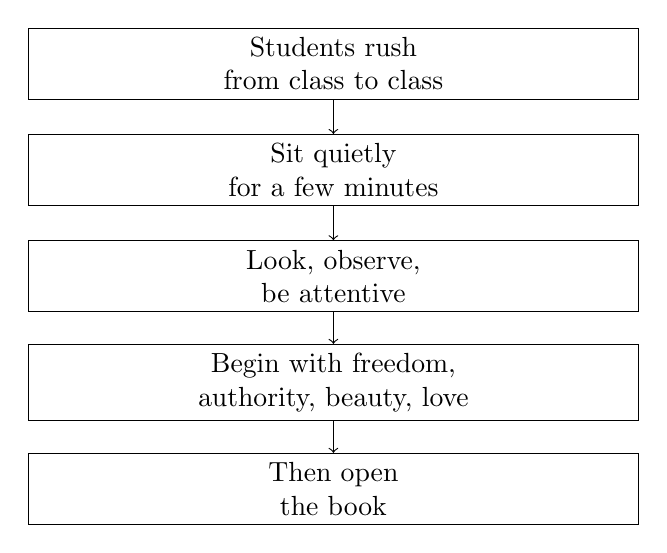
\begin{tikzpicture}
\node[draw, text width=0.62\linewidth, align=center] (a) at (0,0) {Students rush\\from class to class};
\node[draw, text width=0.62\linewidth, align=center] (b) at (0,-1.35) {Sit quietly\\for a few minutes};
\node[draw, text width=0.62\linewidth, align=center] (c) at (0,-2.70) {Look, observe,\\be attentive};
\node[draw, text width=0.62\linewidth, align=center] (d) at (0,-4.05) {Begin with freedom,\\authority, beauty, love};
\node[draw, text width=0.62\linewidth, align=center] (e) at (0,-5.40) {Then open\\the book};
\draw[->] (a) -- (b);
\draw[->] (b) -- (c);
\draw[->] (c) -- (d);
\draw[->] (d) -- (e);
\end{tikzpicture}
\caption{A transcript-based reconstruction of Krishnamurti's classroom order: quiet attention before the book.}
\end{figure}

This is not a method to sell. It is a way of preserving the order of the inquiry. If the book comes first, the student accumulates what others have said. If attention comes first, the book may be seen with what Anderson calls a clean eye.

\subsection{Question \& Answer}

\paragraph{Question.}
How can a book be read without becoming second-hand?

\paragraph{Answer.}
The book must not occupy the first place. If one begins with the book as authority, one accumulates descriptions, traditions, visions of life, and inherited interpretations. If one begins with freedom, quietness, observation, and self-knowing, the book can be used without replacing inquiry.

\begin{align}
\hbox{quiet attention}
\longrightarrow \hbox{self-knowing}
\longrightarrow \hbox{book read with a clean eye}.
\end{align}

Krishnamurti then makes the point more radical. The real book is oneself. If one can read that book, one has learned what matters inwardly, apart from functional knowledge. The external book is not abolished, but it is demoted. It is no longer a substitute for seeing.

\section{The Original Mind And The Real Book}

The word ``second-hand'' gives the next movement its force. A second-hand mind repeats the priest, the scripture, the guru, the philosopher, the teacher, or the inherited formula. Such a mind may have many words about truth, but Krishnamurti insists that reality, if it is real, is original. Therefore the mind that approaches it must be original. By original he does not mean novel, clever, or self-expressive. He means free.

\begin{definition}
An \emph{original mind}, in this lecture, is a mind free enough to look, observe, and learn without dependence on spiritual authority.
\end{definition}

That definition returns us to the central question of religion. Can the mind put aside what human beings have talked about, invented, imagined, and believed about God, religion, truth, saviors, masters, gurus, and scriptures? Can consciousness empty itself of what humanity has said about reality?

Krishnamurti asks this more than once, and the repetition is not filler. Each return removes another hiding place. First there is freedom from the authority of another. Then there is freedom from the structure of thought built around the word religion. Then there is the question whether the mind, heart, and brain can be free of what man has said about reality.

\begin{align}
\hbox{borrowed claim}
&\longrightarrow \hbox{belief},\\
\hbox{belief}
&\longrightarrow \hbox{repetition},\\
\hbox{repetition}
&\longrightarrow \hbox{no discovery}.
\end{align}

This is the negative discipline of the lecture. To put away authority is not to become casual. It is to stop mistaking repetition for discovery.

\section{Leaving The World, Carrying The Baggage}

Krishnamurti then gives the argument a story. In Kashmir, a group of monks tells him about people high in the mountains who have left the world. He asks what that means. If they have left the world, have they left the memory of the world? Have they left the knowledge put together by teachers, gurus, books, sacrifice, torture, and renunciation?

Anderson supplies the image: they went up the mountain with all this baggage. Krishnamurti accepts it. The world can be put away outwardly while being carried inwardly.

\begin{figure}
\centering
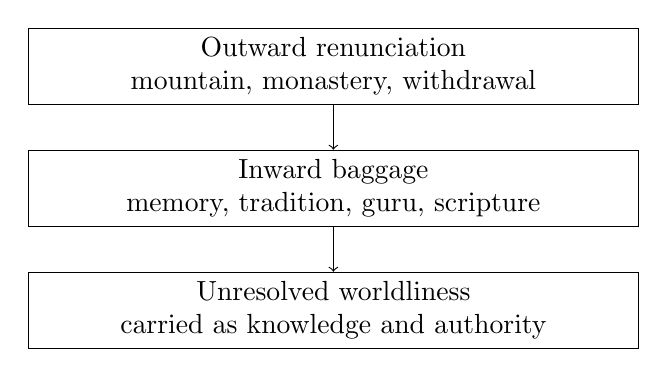
\begin{tikzpicture}
\node[draw, text width=0.62\linewidth, align=center] (a) at (0,0) {Outward renunciation\\mountain, monastery, withdrawal};
\node[draw, text width=0.62\linewidth, align=center] (b) at (0,-1.55) {Inward baggage\\memory, tradition, guru, scripture};
\node[draw, text width=0.62\linewidth, align=center] (c) at (0,-3.10) {Unresolved worldliness\\carried as knowledge and authority};
\draw[->] (a) -- (b);
\draw[->] (b) -- (c);
\end{tikzpicture}
\caption{Outward withdrawal does not by itself free the mind from accumulated memory and authority.}
\end{figure}

The story is not decorative. It prepares the distinction between isolation and aloneness. Isolation can be manufactured by withdrawal, walls, practices, and distance from society. Aloneness, as Krishnamurti uses the word, comes only when the mind has put away the accretions of thought.

\section{Aloneness, Falsehood, And Meditation}

Krishnamurti now asks whether the mind can be completely alone. Not isolated, not withdrawn, not enclosed by a wall, but alone in the sense that all the things of thought have been put away. This brings the lecture to its clearest statement about thought.

Thought, he says, is the response of memory, knowledge, and experience stored in the brain. Therefore thought is of the past. It may function in the field of knowledge; it is necessary there. But thought, being of time, cannot create something that has no time.

\begin{align}
\hbox{memory} + \hbox{knowledge} + \hbox{experience}
&\longrightarrow \hbox{thought},\\
\hbox{thought}
&\longrightarrow \hbox{the past},\\
\hbox{thought of time}
&\not\longrightarrow \hbox{the timeless}.
\end{align}

The last line is a cautious schematic of Krishnamurti's claim. It is not a physical theorem and should not be read as one. It preserves the spoken distinction: thought has a necessary functional place, but it cannot be the instrument of the timeless.

The next move is equally important. Krishnamurti does not ask for bravery, sacrifice, torture, or spiritual heroism. He asks for perception of the false. To see the false is to see the truth in the false; and to see what is conventionally taken as truth as false strips the mind of inward deception.

Desire then enters the inquiry. The desire to experience, to achieve, to arrive, even to become enlightened, creates illusion. Here the lecture gathers earlier discussions of fear, pleasure, and desire into the question of religion.

\begin{align}
\hbox{desire to experience}
&\longrightarrow \hbox{projection},\\
\hbox{projection}
&\longrightarrow \hbox{illusion},\\
\hbox{freedom}
&\longrightarrow \hbox{understanding fear, desire, and pleasure}.
\end{align}

Anderson notices a final danger. One can repeat these questions and think one has grasped them. Krishnamurti's answer is exact: one has grasped the words. The map is not the movement; the phrase is not the perception; the concept is not the act.

The conversation then opens meditation. Religion, in the sense under discussion, and meditation go together. Religion is not an idea or a verbal structure. It is conduct in daily life: thought, speech, behavior, relationship, love, death, and care. Anderson brings in the root sense of meditation as thinking, pondering, going into, and caring for. Krishnamurti sharpens the word from carefulness to caring.

\begin{align}
\hbox{conduct} + \hbox{relationship} + \hbox{love} + \hbox{death} + \hbox{care}
\longrightarrow \hbox{religion and meditation}.
\end{align}

The lecture closes with a social warning. Priests, gurus, business interests, teachers, and politicians all press the mind back into dependence. They have their vested interests. The next inquiry, meditation, must be taken up within that whole field, not outside it.

\section{Summary}

The conversation unfolds as a sequence of increasingly exact questions. First, why do we come to the brink of inquiry and run away? Then, how has education in function and measure trained the mind to depend on authority? Then, can there be inquiry without freedom from the beginning? Then, can books, scriptures, and inherited knowledge be used without making the student second-hand?

The second half deepens the same movement. The original mind is the free mind. The real book is oneself. Outward withdrawal is not freedom if the mind carries inward baggage. Aloneness is not isolation, and thought, though necessary in the field of knowledge, cannot govern the inquiry into the timeless. To see the false is not an act of violence or self-torture; it is the beginning of inward clarity. Desire for spiritual achievement produces illusion. Religion, finally, is not belief or institution but the regeneration of life through attention, conduct, relationship, love, death, and care. Meditation is the next question opened by that whole movement.